\documentclass[a4paper,12 pt]{article}
\usepackage[slovene]{babel}
\usepackage[utf8]{inputenc}
\usepackage[T1]{fontenc}
\usepackage{lmodern}
\usepackage{graphicx}
\usepackage{amssymb}
\usepackage{hyperref}
\usepackage[top=1.3in, bottom=1.3in, left=1.25in, right=1.25in]{geometry}

\begin{document}
\begin{titlepage}
\begin{center}

\large
Univerza v Ljubljani\\
\normalsize
Fakulteta za matematiko in fiziko\\

\vspace{3 cm} 

\large
Eva Deželak, Žan Jarc, Veronika Sovdat in Ines Šilc\\

\vspace{0.5cm}
\LARGE
\textbf{Kazalniki ekonomske neenakosti}

\vspace{0.5 cm}
\normalsize
Seminar

\vspace{1.5cm}
\normalsize
Mentor: doc. dr. Matija Vidmar

\vspace{3cm}


\vfill

\large Ljubljana, 2019

\end{center}
\end{titlepage}

\newpage

\tableofcontents
\vspace{20mm}

\newpage

\section[Uvod]{Uvod}

\subsection[Definicije osnovnih pojmov]{Definicije osnovnih pojmov}
Za začetek si poglejmo nekaj pojmov, na katere pogosto zasledimo ob raziskovanju ekonomske neenakoti.
\\ 

\textbf{Državni dohodek} je vsota vseh dohodkov, ki so na voljo prebivalcem neke države v danem letu, ne glede na klasifikacijo dohodkov. Državni dohodek je povezan z bruto domačim proizvodom, vendar ne predstavljata enakih prihodkov. Bruto domači proizvod meri vsoto dobrin in sredstav, proizvedenih v enem letu znotraj meja neke države. Da dobimo državni dohodek, moramo od BDP odšteti ceno kapitala potrebnega za nastanek dobrin in sredstev. Odšteti moramo torej infrastrukturo, vozila, računalnike...). Ko to odštejemo, dobimo \textbf{neto} domači proizvod. Temu dodamo še neto dobičke iz tujine, da dobimo državni dohodek.
$$
\textbf{Državni dohodek} = \textbf{BDP} - \textbf{cena kapitala} + \textbf{neto dobiček iz tujine}
$$
V večini držav državni dohodek predstavlja od $1\%$ do $2\%$ bruto domačega proizvoda, to pomeni, da je dohodek sorazmeren z odhodkom. V bogatejših državah je neto dohodek ponavadi pozitiven, torej prebivalci te države si lastijo enako tujih posestvi in finančnih inštrumentov, kot si jih tujci pri njih.

Državni dohodek je lahko višji ali manjši od BDP, odvisno od neto dohodka iz tujine, torej če je ta pozitiven ali negativen.
\\

\textbf{Kapital} predstavljajo vse oblike dejanske lastnine in profesionalnega kapitala (sem spadajo na primer patenti, ki niso fizična, ampak intelektualna lastnina), ki ga uporabljajo podjetja in javne agencije. Tu izločujemo \textbf{človeški kapital}, ki se razume kot zmožnost nekega posameznika in njegove spretnosti. Človeškega kapitala si ne moremo lastiti.
\\

\textbf{Državno premoženje} je vsota privatnega in javnega premoženja. Javno premoženje ponavadi zanemarimo, saj je velikokrat negativno. To se zgodi, če je javni dolg večj kot javna lastnina, zato državno premoženje večinoma predstavlja privatno premoženje državljanov.
$$
\textbf{Državno premoženje}=\textbf{državni kapital}=\textbf{domači kapital}+\textbf{neto tuji kapital}
$$
Domači kapital je vrednost kapitalskih delnic (gradbenih objektov, podjetij...), ki se nahajajo znotraj neke države. Neto tuji kapital, ali \textbf{neto tuja lastnina}, pa meri pozicijo države v primerjavi s preostalim svetom. Natančneje, je razlika med lastnino, ki je v lasti državljanov v tujini in lastnino tujih državljanov v prvotni državi.
\newpage

\subsection[Neenakost v odnosu do dela in kapitala]{Neenakost v odnosu do dela in kapitala}

Dohodek lahko prihaja iz dela ali pa iz kapitala. Plače so ena oblika dohodka iz dela, dohodek iz kapitala pa predstavlja vse prihodke, ki jih ima lahko nek posameznik od kapitala, to so lahko na primer najemnine, dividende, obresti\dots. Definiramo \textbf{dohodkovo neenakost} kot vsota neenakosti dohodka iz dela in kapitala.

Dohodek iz dela večkrat enačimo s plačami in kot kazalnik ekonomska neenakost večkrat vzamemo razlike v plačah. Tu se najpogosteje pojavi teorija o tekmi med izobraževanjem in tehnologiji.

\subsubsection[Tekma med izobraževanjem in tehnologijo]{Tekma med izobraževanjem in tehnologijo}

Teorija ima dve predpostavki:
\begin{enumerate}
\item Plača delavca je enaka njegovi \textbf{mejni produktivnosti}, kjer mejna produktivnost predstavlja prispevek delavca k njegovem delodajalcu.
\item Produktivnost delavca je odvisna od njegovih spretnosti in strokovnega znanja ter \textbf{ponudbi} teh spretnosti v dani družbi.
\end{enumerate}

Teorija o tekmi med izobraževanjem temelji predvsem na ponudbi in povpraševanju strokovnega znanja v neki državi. Ponudba prihaja iz izobraževalnega sistema, medtem ko je povpraševanje odvisno od razpoložljive tehnologije, ki je na voljo za proizvajanje dobrin in storitev, potrebnih v dani družbi.

Tehnološki napredek je odvisen od hitrosti inovacij in hitrosti implementacije teh inovacij. Ponavadi dvigne povpraševanje za nova strokovna znanja in ustvari nova delovna mesta. Tu nastane t.i. tekma, saj če se ponudbe delavcev s primernimi strokovnimi znanji ne poveča hkrati z tehnologijo, bodo nastale skupine ljudi, katerih znanje ni zadovoljivo. Te skupine bodo zaslužile manj in njihovo delo se bo razvrednotilo. Tako pride do neenakosti v plačah.

Ta teorija ima predvsem dve veliki \textbf{pomanjkljivosti}:
\begin{enumerate}
\item Plača seveda ni perfektno določena z mejno produktivnostjo, spretnostmi in strokovnimi znanji danega delavca.
\item Ne razloži gromozanskih razlik med plačami direktorjev in delavci podjetja.
\end{enumerate}


\newpage

\section[Posamezni kazalniki]{Posamezni kazalniki}
\subsection[Prag revščine]{Prag revščine}

\subsection[Ginijev koeficient]{Ginijev koeficient}
Ginijev koeficient je merilo neenakomerne porazdelitve sredstev med populacijo. Imenuje se po italijanskem statistiku Corradu Giniju (1884-1965). Nižji kot je koeficient,  bolj enakomerna je porazdelitev,  in višji kot je,  bolj neenakomerna je porazdelitev. Zavzame lahko vrednosti med 0 (popolna enakost) in 1 (eden ima vse). Torej število 0 predstavlja popolno enakost (vsakdo ima popolnoma enaki prihodek in premoženje), število 1 pa predstavlja popolno neenakost (nobeden nima enakega prihodka in premoženja). 

Tipičen primer neenakomerne porazdelitve premoženja predstavlja podatek, da si 10 \% svetovnega prebivalstva lasti 87, 7 \% celotnega svetovnega bogastva.

\subsection[Lorenzova krivulja]{Lorenzova krivulja}

Ginijev  koeficient  definiramo  s  pomočjo  Lorenzove  krivulje,  ki  je  grafični  prikaz porazdelitve neke količine med prebivalstvom.

Denimo,  da  je  med  populacijo  velikosti  N  porazdeljena  količina  Q,  ki  na  primer  predstavlja  družinski  dohodek,  premoženje,  zemljo  ...   Populacijo  razvrstimo po naraščajočem vrstnem redu njihovega deleža količine  Q.  Za vsak p med 0 in 1 ljudje v prvem p-tem deležu predstavljajo najrevnejših (glede na Q) 100p odstotkov populacije.   Z  L(p)  označimo  del  količine  Q,  ki  si  jo  lasti  ta  del  populacije. Tako smo podali funkcijo L, ki preslika interval [0, 1] vase. Njen graf imenujemo Lorenzova  krivulja. 

V primeru, da bi si vsak posameznik lastil enak delež količine Q, bi bila  enačba  Lorenzove  krivulje  $L(p)  =  p$  in  bi  predstavljala  popolno  enakomerno porazdelitev premoženja.  Iz definicije funkcije L sledi, da je $0 \leq L(p) \leq p$ za vsak $p \in [0, 1]$. 

\begin{figure}
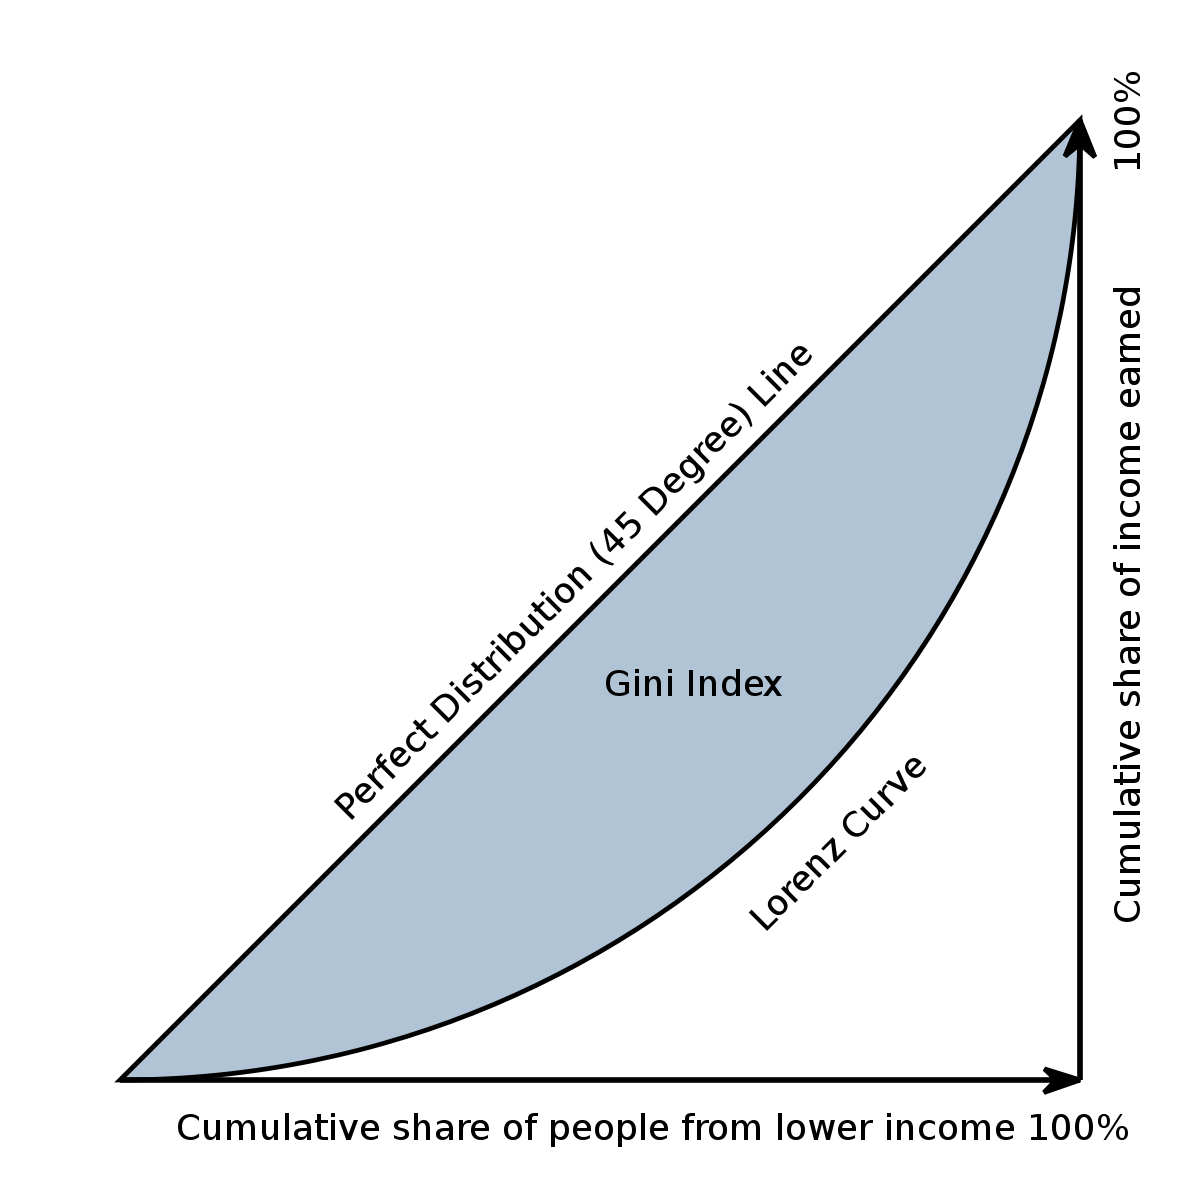
\includegraphics[width= \linewidth]{./slike/lorenzova-krivulja.png}
\end{figure}

Ginijev koeficient je dvakratnik ploščine med grafom popolne enakomerne porazdelitve in med grafom Lorenzove krivulje.

Ginijev koeficient je torej količina, izračunana iz Lorenzove krivulje: 
$$G := 2 \cdot \int_{0}^{1} (p - L(P)) dp. $$

Ker je $0 \leq \int_{0}^{1} (p - L(P)) dp \leq \int_{0}^{1} p dp = \frac{1}{2}$, je $G \in [0, 1].$

\begin{figure}
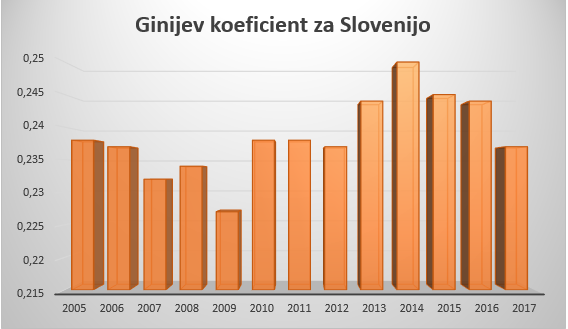
\includegraphics[width= \linewidth]{./slike/gini-slo.png}
\end{figure}

\begin{figure}
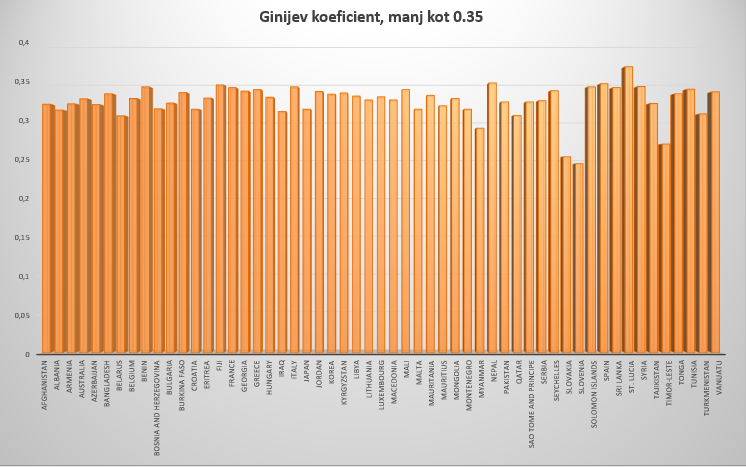
\includegraphics[width= \linewidth]{./slike/gini-manj-07.png}
\end{figure}

\begin{figure}
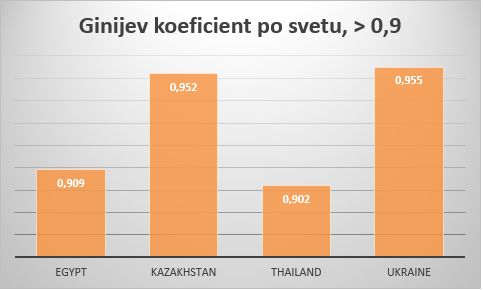
\includegraphics[width= \linewidth]{./slike/gini-vec-09.png}
\end{figure}

\subsection[Palmovo razmerje]{Palmovo razmerje}

\newpage

\section[Ekonomska neenakost doma in po svetu]{Ekonomska neenakost doma in po svetu}

\newpage

\section[Ekonomska neenakost in demokracija]{Ekonomska neenakost in demokracija}

\newpage

\section[Viri]{Viri}

\begin{itemize}
\item
\label{Pickety}
T.~Pickety, \emph{Capital in the twenty-first century}, The Belknap Press of Harvard University Press, London, 2014.

\item 
\label{Razdelitev premoženja}
\emph{Distribution of wealth}, v: Wikipedia, The Free Encyclopedia, [ogled 20.~4.~2019], dostopno na \url{https://en.wikipedia.org/w/index.php?title=Distribution_of_wealth&oldid=854198883}.

\item 
\label{Metrike ekonomske neenakosti}
\emph{Income inequality metrics}, v: Wikipedia, The Free Encyclopedia, [ogled 20.~4.~2019], dostopno na \url{https://en.wikipedia.org/w/index.php?title=Income_inequality_metrics&oldid=853906711}.

\item
\emph{Ginijev koeficient}, Janja Trogar, [ogled 3.~5.~2019], dostopno na \url{https://repozitorij.uni-lj.si/IzpisGradiva.php?id=97164}.

\item
\emph{Statistični urad RS}, Neenakost porazdelitve dohodka - Ginijev količnik (\%), Slovenija, letno, [ogled 4.~5.~2019], dostopno na \url{https://pxweb.stat.si/pxweb/Dialog/varval.asp?ma=0867312S&ti=&path=../Database/Dem_soc/08_zivljenjska_raven/08_silc_kazalniki_revsc/15_08673_porazdel_dohodka/&lang=2}.
\end{itemize}

\end{document}